%% The first command in your LaTeX source must be the \documentclass command.
%%
%% Options:
%% twocolumn : Two column layout.
%% hf: enable header and footer.
\documentclass[
twocolumn,
% hf,
]{ceurart}

%%
%% One can fix some overfulls
\sloppy

%%
%% Minted listings support 
%% Need pygment <http://pygments.org/> <http://pypi.python.org/pypi/Pygments>
\usepackage{listings}
%% auto break lines
\lstset{breaklines=true}

\usepackage{blindtext}
\usepackage[linesnumbered,ruled]{algorithm2e}
\usepackage{amsmath}
\usepackage{tikzsymbols}
\usepackage{pifont} % for \ding command
\usepackage{listings}
\usepackage{multirow}
\usepackage{bm}
\usepackage{bbm}
\usepackage{xfrac}
\usepackage{booktabs} % For better horizontal rules
\usepackage{cellspace} % For adjusting vertical spacing
\usepackage{xcolor}
\newcommand\todop[1]{\textcolor{red}{#1}} % todo in the paper
\newcommand\todos[1]{\textcolor{blue}{#1}} % todo in the software
\newcommand{\tik}{\textcolor{green}{\ding{51}}}
\newcommand{\ntik}{\textcolor{red}{\ding{55}}}
\usepackage{lastpage}
\usepackage{caption}
\usepackage{subcaption}

\newcommand{\xcc}{\mathbf{x_{/s}}}
\newcommand{\Xcal}{\mathcal{X}}
\newcommand{\xb}{\mathbf{x}}
\newcommand{\xc}{\mathbf{x_c}}
\newcommand{\Xc}{\mathbf{X_c}}
\newcommand{\xci}{\mathbf{x}^i_c}



%%
%% end of the preamble, start of the body of the document source.
\begin{document}

%%
%% Rights management information.
%% CC-BY is default license.
\copyrightyear{2024}
\copyrightclause{Use permitted under Creative Commons License Attribution 4.0 International (CC BY 4.0).}

%%
%% This command is for the conference information
\conference{The 2nd World Conference on eXplainable Artificial Intelligence,
  July 17--19, 2024, Malta, Valetta}

%%
%% The "title" command
\title{Fast and accurate regional effect plots for inspecting black-box models fit on tabular data}

%%
%% The "author" command and its associated commands are used to define
%% the authors and their affiliations.
\author[1,2]{Vasilis Gkolemis}
\address[1]{Harokopio University of Athens}
\address[2]{ATHENA Research Center}
\author[1]{Christos Diou}
\author[3]{Eirini Ntoutsi}
\address[3]{University of the Bundeswehr Munich}
\author[2]{Theodore Dalamagas}
\author[4]{Bernd Bischl}
\address[4]{Munich Center for Machine Learning (MCML), Department of Statistics, LMU Munich}
\author[4]{Julia Herbinger}
\author[4]{Giuseppe Casalicchio}


\begin{abstract}
  The regional effect is a novel explainability method that can be used to extract insights from tabular data through a three-step procedure; a black-box machine learning model is trained on a tabular dataset, a regional effect method explains its learnings, and the explanations are used to understand the data and and support decision making.
  Regional effect methods explain each feature within different subgroups, such as how age (feature) affects annual income (output) for men and women separately (subgroups). However, identifying significant subgroups automatically is computationally intensive, and current regional effect methods face efficiency challenges.
  In this paper, we introduce rRHALE (regional RHALE), a method that overcomes these issues. rRHALE is notably more efficient compared to existing regional effect approaches, making it suitable for large datasets and complex models. It also handles well cases where the inputs features are highly-correlated. We demonstrate the advantages of rRHALE through a set of synthetic examples, where we compare it to other regional effect methods, and apply  rRHALE to a real-world scenario. The supporting code for this publication is available.
\end{abstract}

%%
%% Keywords. The author(s) should pick words that accurately describe
%% the work being presented. Separate the keywords with commas.
\begin{keywords}
  Explainability \sep
  Interpretability \sep
  Feature Effect \sep
  Regional Effect \sep
  Global Explanations
\end{keywords}

%%
%% This command processes the author and affiliation and title
%% information and builds the first part of the formatted document.
\maketitle


\section{Introduction}
\label{sec:introduction}

% In recent years, the notable surge in available data has increased the need for automated data analytics tools.
Recently, there has been significant progress in Machine Learning (ML) on tabular data, with models able to learn data patterns and execute tasks like prediction. Although, most of these models operate as black-boxes, i.e., they take inputs and produce outputs with opaque inner workings, eXplainable AI (XAI) has emerged to explain how they operate. Combining Machine Learning with XAI offers a promising avenue for data analysis. As shown in Figure~\ref{fig:concept_figure}, the idea is to understand the data at hand by explaining the black-box model that is trained on them.

To better grasp the concept consider the bike-sharing dataset, that contains a set of features such as the temperature, the humidity, the hour of the day, whether it is a working day or weekend etc, and we want to predict the bike-rentals on an hour-basis.

We the final goal to understand the tabular data and support decision making, we apply the following pipeline. First, we fit a black-box model, like a neural network or a decision tree. Then, we apply a regional effect to understand the effect of hour on the ouput. The regional effect explains that for working days, there are two sharp rises in bike-rentals at about 8:30 AM and 17:00 AM, when people go to and return from work. For non-working dayes, bike rentals increase from 9:00 AM, reach a peak at 12:00 AM and a decline at 4:00 PM, which a typical use for sigthseeing. Equivalent work can be done for all other features one after the other.

Such analysis provides insights for decision making; the owner of the bike shop can apply an offer on different hours on weekens and working days.


Regional effect methods automatically identify the meaningful subregions (male/female) which is computationally demanding. They internally compute heterogeneity, a quantity tha shows how much local effects deviate from the average effect, and search for a split that minimizes it. Since such search in the input space requires iterating over all features and thets the heterogeniety of each split.

Current regional effect methods, namelly ..., face efficicent issurs, they runs efficiently on problems with heavy models, high-dimensional and big datasets. Therefore, we present rRHALE, a regional effect method that overcomes these problems.

\begin{itemize}
\item is very fast making it feasible to apply it on cases where the model is highly-dimentiosnl.
\item handles well cases with correalted features, avoiding to create out of out of distribution sampling.
\item demonstrates through tutorials the use of regional effects in real and synthetic datasets.
\end{itemize}

\begin{figure*}[t]
    \centering
    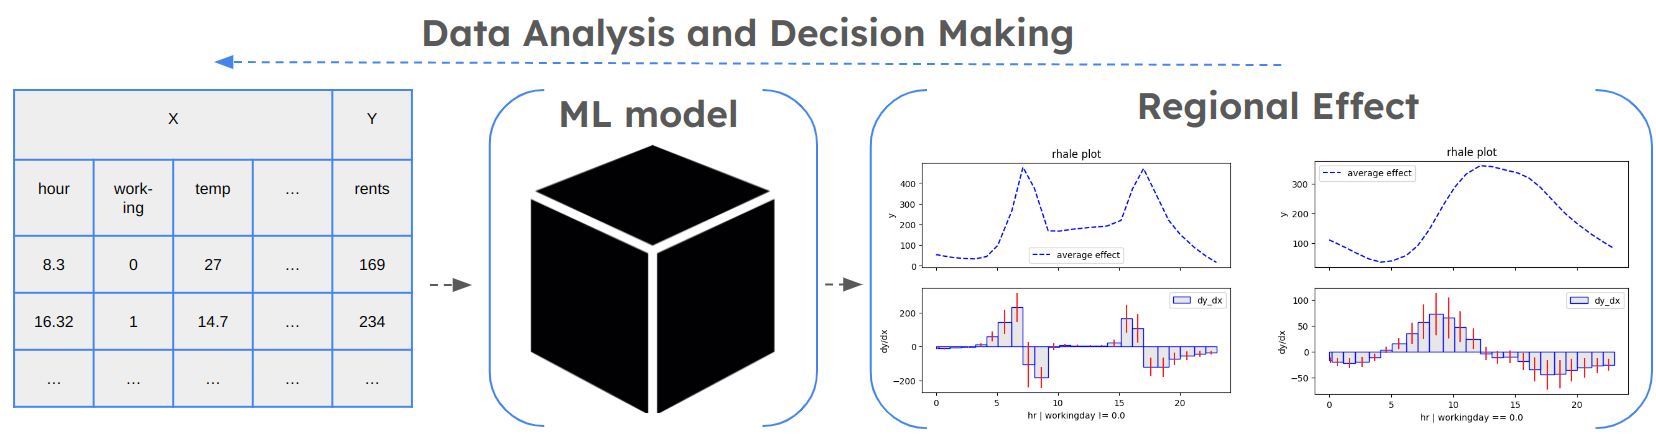
\includegraphics[width=\textwidth]{figures/concept_image.png}
    \caption{Data analysis and decision making pipeline: Utilizing regional effect plots to extract insights from tabular data.}
    \label{fig:concept_figure}
\end{figure*}

\section{Regional RHALE}


rRHALE is the regional version of RHALE, a global effect method for differentiable black-box models. It builds on two key papers. The first, by Gkolemis et al. (2023)~\citep{gkolemis2023rhale}, introduced RHALE which improves ALE by incorporating automatic bin splittingfor unbiased heterogeneity estimation. The second paper, by Herbinger et al. (2023)~\citep{herbinger2023decomposing}, proposed a framework for transforming regional effect methods from global and applied it to PDP, ALE, and SHAP-DP.

\subsection{Method Description}

\paragraph{Notation.}

Let \(\mathcal{X} \in \mathbb{R}^d\) be the \(d\)-dimensional feature space, \(\mathcal{Y}\) the target space and
\(f(\cdot) : \mathcal{X} \rightarrow \mathcal{Y}\) the black-box function.
We use index \(s \in \{1, \ldots, d\}\) for the feature of interest and \(/s = \{1, \ldots, d\} - s\) for the rest.
For convenience, we use \((x_s, \xc)\) to denote the input vector \((x_1, \cdots , x_s, \cdots, x_D)\),
\((X_s, \Xc)\) instead of \((X_1, \cdots , X_s, \cdots, X_D)\) for random variables and
$\mathcal{X}_s, \mathcal{X}_{c}$ for the feature space and its complement, respectively.
The training set \(\mathcal{D} = \{(\xb^i, y^i)\}_{i=1}^N\) is sampled
i.i.d.\ from the distribution \(\mathbb{P}_{X,Y}\).

\paragraph{RHALE global effect.}

RHALE resolves that by approximating the global effect as:

\begin{equation}
  \label{eq:rhale-approximation}
\hat{f}^{\mathtt{RHALE}}(x_s) = \sum_{k=1}^{k_{x_s}} \underbrace{\frac{z_k - z_{k-1}}{ \left | \mathcal{S}_k \right |} \sum_{i: \xb^i \in \mathcal{S}_k} \frac{\partial f}{\partial x_s} (x_s^i, \xci)}_{\hat{\mu}_k^{\mathtt{RHALE}}}
\end{equation}

\noindent
RHALE's \textit{approximation} differentiates from ALE \textit{approximation} in two aspects. First, it computes the derivative effects using automatic differentiation instead of finite differences at the bin limits. This estimates the derivative effects more accurately and faster~\citep{gkolemis22a, gkolemis2023regionally}. Second, it automatically partitions the $s$-th axis into a sequence of $K_s$ variable-size intervals, i.e., $\{\mathcal{Z}_k\}_{k=1}^{K_s}$. Each interval covers a range from $z_{k-1}$ to $z_k$, and defines the set $\mathcal{S}_k$ with the instances that lie inside, i.e., $\mathcal{S}_k = \{ x^{(i)} : z_{k-1} \leq x^{(i)}_s < z_k \}$. The automatic bin-splitting is performed by solving an optimization problem that minimizes the heterogeneity of the derivative effect within each bin~\citep{gkolemis2023rhale}.

\paragraph{Heterogeneity}

The \textit{approximations} of the heterogeneity index is given by:

\begin{equation}
  \label{eq:rhale-approximation-heterogeneity}
  \hat{H}_s^{\mathtt{RHALE}} = \sum_{k=1}^{K_s} \frac{z_k - z_{k-1}}{|\mathcal{S}_k|}\sum_{i: \xb^i \in \mathcal{S}_k} \left [ \frac{\partial f}{\partial x_s} (x_s^i, \xci) - \hat{\mu}_k^{\mathtt{RHALE}} \right ]^2
\end{equation}

\paragraph{Regional RHALE}

The regional RHALE is 


\subsection{Computational Complexity}

All regional effect methods follow the CART-based approach of Algorithm(add reference), with computational complexity of ... Algorithm(cite) executes the prediction function $(D-1) \times N_2 $ for computing the best split on a particular level, leading to a total of $(D-1) \times N_2 \times M$ execution of f.

\clearpage
\section{Syntetic Examples}

We generate two synthetic examples: one demonstrates that rRHALE is significantly faster than rPDP and rALE, and the other that rRHALE, handles well tabular datasets with correlated features, unlike rPDP.

\section{Efficiency}

In these examples, we will show that rRHALE is faster than rPDP and rALE. Specifically, it executes fast even under a (a) slow-inference black-box model and (b) a large tabular dataset.

\paragraph{Slow-inference black-box model:}

We generate a synthetic dataset with $N=10^4$ instances and $D=10$ features. Then, we train deep neural networks (DNN) with number of layers ranging from $L=3$ to $L=20$. Larger neural networks lead to increased inference times, so our findings generalize to all set-ups where the underlying model has slow inference.

In Figure~\ref{fig:efficiency_heavy_model}, we show that rRHALE's execution time stays almost constant independenly of the models inference time.
Therefore, even for a heavy model, such as a DNN with $20$ layers, needs less than than 15 seconds to create regional effect plots for one feature, which leads to a few minutes (4-5 minutes) for a typical tabular dataset, like $D=20$. In contrast, PDP would need about 4 minutes per feature, so about an hour for all features, and ALE about 1 minute so about 20 minutes for alla features.

\paragraph{Large tabular dataset}

We create a DNN with $L=5$ layers and a synthetic dataset with $D=20$ features and number of instances ranging in $N \in \{10^3, 10^4, 10^5\}$ (log scale).

In Figure~\ref{fig:efficiency_nof_instances}, we show that rRHALE's is the fastest approach as the number of instances increases. rRHALE is more than $x2$ faster than ALE and $x10$ than PDP, which for large datasets corresponds to a speed-up of $20$ minutes compared to rALE and 2 hours compared to rPDP. Also, notice that the effect would be even more pronounced if the model was heavier, as shown in the previous example.

\begin{figure}
    \centering
    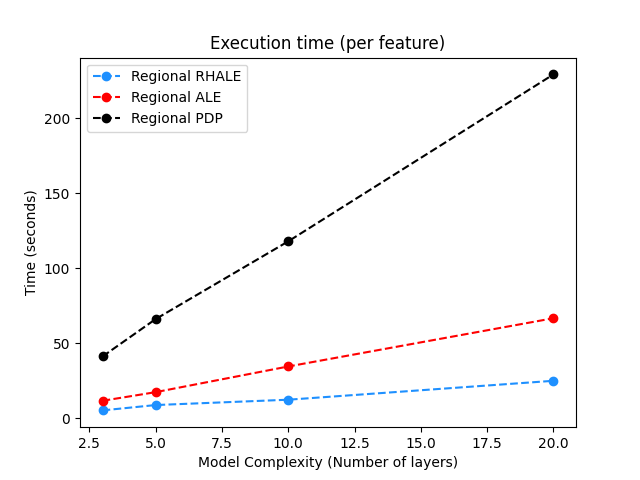
\includegraphics[width=.49\textwidth]{figures/simulation_2/efficiency_layers.png}
    \caption{Data analysis and decision making pipeline: Utilizing regional effect plots to extract insights from tabular data.}
    \label{fig:efficiency_heavy_model}
\end{figure}

\begin{figure}
    \centering
    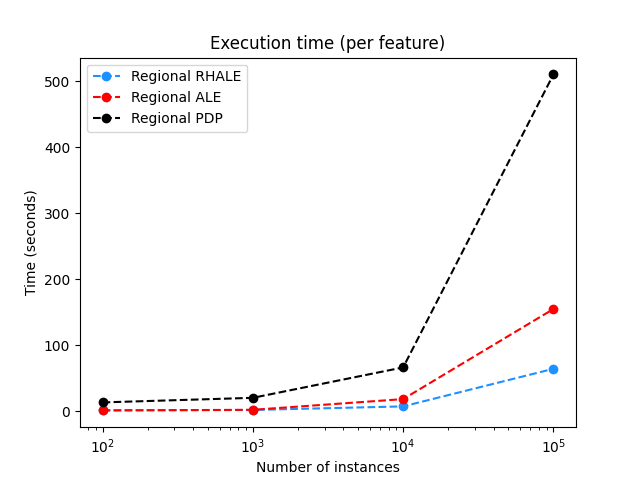
\includegraphics[width=.49\textwidth]{figures/simulation_2/efficiency_samples.png}
    \caption{Data analysis and decision making pipeline: Utilizing regional effect plots to extract insights from tabular data.}
    \label{fig:efficiency_nof_instances}
\end{figure}


\section{Correlated Features}

The purpose of this example is to shwocase the superiority of Regional RHALE compared to Regional PDP, when features are correlated. In such cases, Regional PDP may erroneously find subregions due to out of distribution sampling.

Consider a black-box function $y = 3x_1I_{x_3>0} - 3x_1I_{x_3\leq0} + x_3$ and two different setting for the data generating distribution. In the non-correlated setting, all variables are uniformly distributed, i.e., $x_i \sim \mathcal{U}(-1,1)$.
In the correlated setting, we keep the same distributions for $x_1$ and $x_2$, but we set $x_3 = x_1$. We will focus on the effect (global and regional) of $x_1$ on $y$.

\paragraph{correlated setting.}

The effect of $x_1$ is provoked by the interaction terms, i.e., $3x_1I_{x_3>0}$ and $3x_1I_{x_3\leq0}$. The global effect will be $3x_1$ when $x_3>0$ (half of the times considering that $x_3 \sim \mathcal{U}(-1,1)$) and $-3x_1$ when $x_3 \leq 0$ (the other half). This results in a zero global effect with high heterogeneity. If splitting into two subregions, $x_3>0$ and $x_3 \leq 0$, we get two regional effects, $3x_1$ and $-3x_1$, with zero heterogeneity each. In figure~\ref{fig:synthetic-1-uncorrelated}, we observe that both rPDP and rRHALE find correctly both global and regional effect.




\begin{figure*}[t]
    \centering
    \begin{subfigure}[b]{0.33\textwidth}
        \centering
        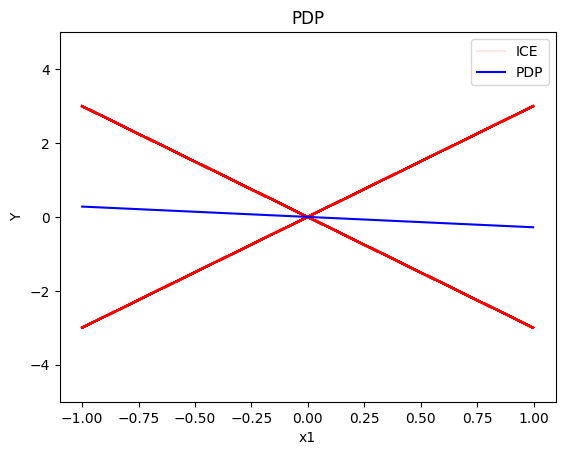
\includegraphics[width=\textwidth]{figures/simulation_1/uncor_global_pdp.png}
        \caption{Global PDP ($x_1$)}
        \label{subfig:a}
    \end{subfigure}
    \begin{subfigure}[b]{0.33\textwidth}
        \centering
        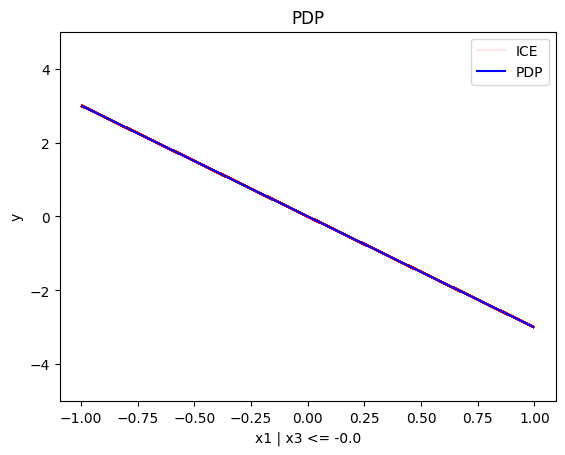
\includegraphics[width=\textwidth]{figures/simulation_1/uncor_regional_pdp_1.png}
        \caption{Regional PDP ($x_1 | x_3 \leq 0$)}
        \label{subfig:b}
    \end{subfigure}
    \begin{subfigure}[b]{0.33\textwidth}
        \centering
        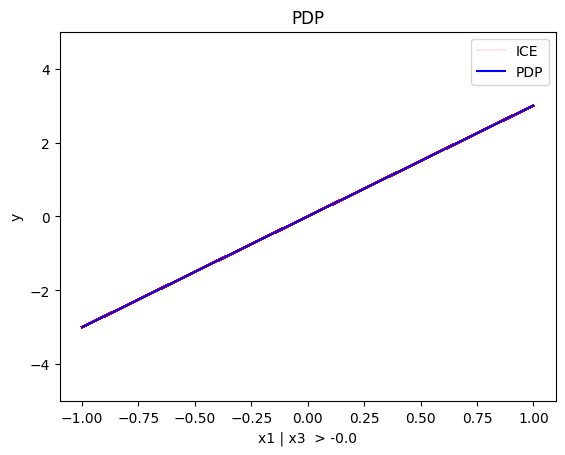
\includegraphics[width=\textwidth]{figures/simulation_1/uncor_regional_pdp_2.png}
        \caption{Regional PDP ($x_1 | x_3 > 0$)}
        \label{subfig:b}
    \end{subfigure}
    \begin{subfigure}[b]{0.33\textwidth}
        \centering
        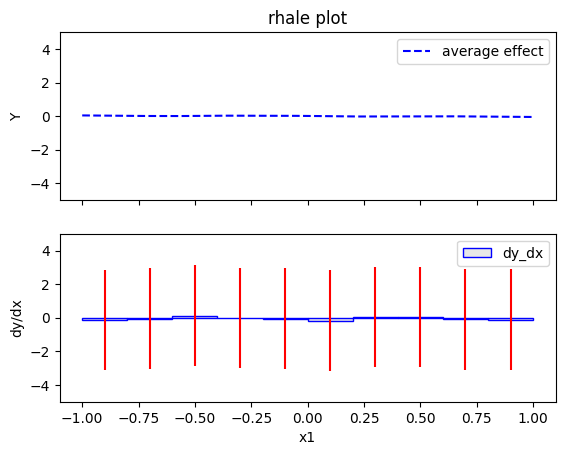
\includegraphics[width=\textwidth]{figures/simulation_1/uncor_global_rhale.png}
        \caption{Global RHALE ($x_1$)}
        \label{subfig:a}
    \end{subfigure}
    \begin{subfigure}[b]{0.33\textwidth}
        \centering
        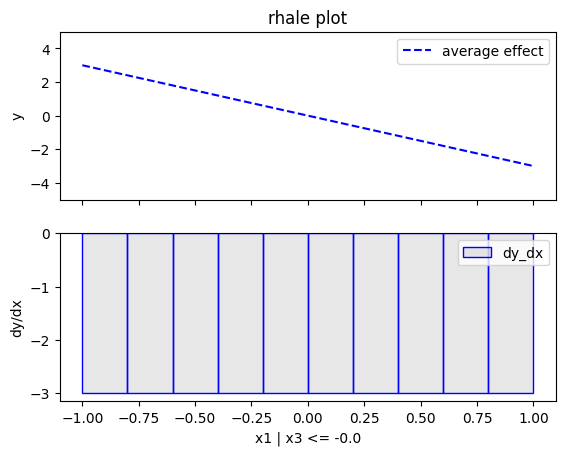
\includegraphics[width=\textwidth]{figures/simulation_1/uncor_regional_rhale_1.png}
        \caption{Regional RHALE ($x_1 | x_3 \leq 0$)}
        \label{subfig:b}
    \end{subfigure}
    \begin{subfigure}[b]{0.33\textwidth}
        \centering
        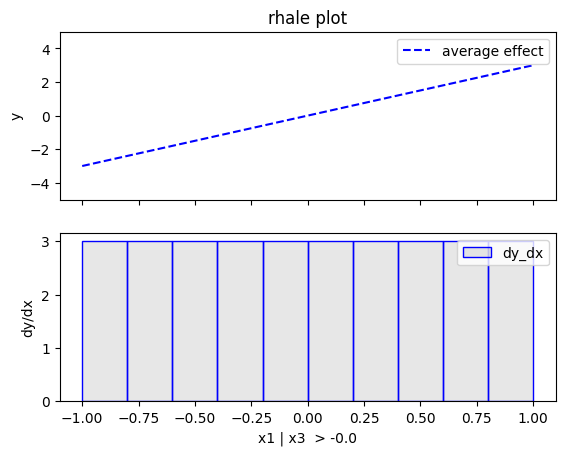
\includegraphics[width=\textwidth]{figures/simulation_1/uncor_regional_rhale_2.png}
        \caption{Regional RHALE ($x_1 | x_3 > 0$)}
        \label{subfig:b}
    \end{subfigure}
    \caption{Global and regional effect for the uncorrelated setting of synthetic example 1, using PDP and RHALE methods.}
    \label{fig:synthetic-1-uncorrelated}
  \end{figure*}

\paragraph{Correlated setting.}

  In the correlated case, due to $x_3=x_1$, the interaction terms can be written as $3x_1I_{x_1>0}$ and $-3x_1I_{x_1 \leq 0}$.
  This is because when $x_1>0$, $x_3>0$, so only the term $3x_1$ is active. Similarly, when $x_1\leq 0$, $x_3 \leq 0$, making the term $-3x_1$ active.

\begin{figure*}[t]
    \centering
    \begin{subfigure}[b]{0.49\textwidth}
        \centering
        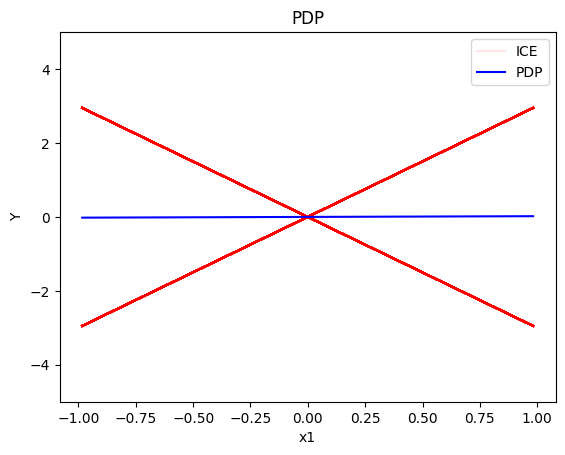
\includegraphics[width=\textwidth]{figures/simulation_1/cor_global_pdp.png}
        \caption{Global effect}
        \label{subfig:a}
    \end{subfigure}
    \begin{subfigure}[b]{0.49\textwidth}
        \centering
        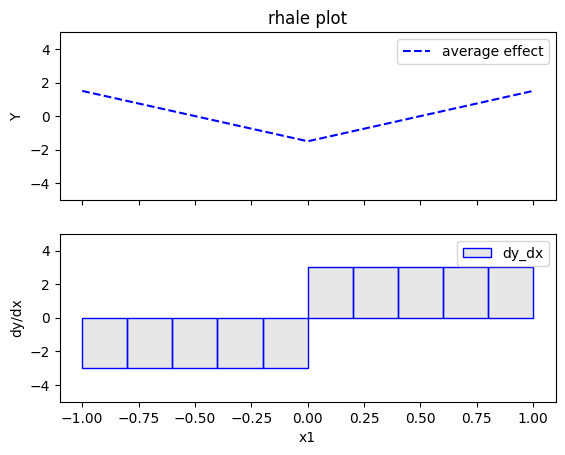
\includegraphics[width=\textwidth]{figures/simulation_1/cor_global_rhale.png}
        \caption{Global effect}
        \label{subfig:a}
    \end{subfigure}
    \caption{Global and interaction effects.}
    \label{fig:main-concept}
  \end{figure*}
  
  
\section{Conclusion and Future Work}

\bibliography{regional_rhale.bib}

\end{document}

%%
%% End of file
